\chapter{Návrh architektury}
\label{chap:architecture}

Aplikace se skládá ze dvou hlavních celků, webového klienta a serveru. Většina logiky je na straně klienta, server slouží pouze pro načítání dat z datastore.

\section{Server}

Server je minimální, chová se jako prostředník mezi datastore a klientem. Jeho součástí je modul pro souborový systém, pomocí něhož je možné procházet adresáře a vypisovat přítomné datastory. Model API načítá neurony v jednotlivých vrstvách a jejich spojení. ADS API pak načítá seznam a detaily datových struktur. Jak modelová část serveru, tak ADS část serveru kromě veřejného rozhraní zahrnují jen minimální transformaci dat do formátu vhodného pro frontend.

\begin{figure}
  \centering
  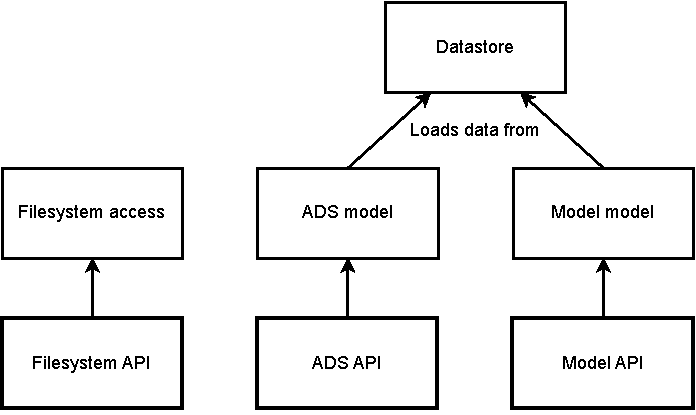
\includegraphics[width=.7\linewidth]{img/server_diagram.pdf}
  \caption{Architektura serveru}
\end{figure}

\subsection{Popis API}

Původní záměr byl vybudovat klasické JSON API. Během vývoje se ale ukázalo, že nejde o proveditelný nápad. Model i ADS zprávy mohou narůst do ohromné velikosti (například spojení mezi dvěma vrstvami mohou být desítky milionů). Když se server pokoušel zakódovat do JSON pole takových rozměrů, narazil na limit přidělené paměti. Jako JSON se tedy posílají jen relativně krátké zprávy, většinou metadata. Hlavní objem dat se streamuje ve formátu CSV. To má benefit i v lepším využití času na straně frontendu --- data se mohou začít zpracovávat už během stahování.

Speciální případ je načítání detailu ADS. Různé druhy ADS mají různě strukturovaná data s velkým objemem. Liší se jak dimenzionalita polí, tak jejich počet. API je vytvořené tak, aby frontend tyto informace nemusel předem znát. Detail API, který frontend dostane, místo některých properties může obsahovat \lstinline|@link| objekty. Ty frontendu sdělí, na jaké URI nalezne daná streamovaná data a jakou mají strukturu. Frontend si pak data automaticky nalezne sám. Rozměry CSV tabulky streamovaných ADS dat nemusí odpovídat rozměrům výsledného pole --- u více než dvourozměrného pole by to ani nebylo možné. Frontend si vytvoří prázdné pole správných rozměrů a do něj sekvenčně vyplňuje přijímaná data. Přidání nového druhu ADS tedy znamená změny v API pouze na straně serveru, načítací service v klientovi se měnit nemusí.

Trochu nešťastné je, že ADS nemají v datastore přiřazený žádný unikátní identifikátor. Jediný způsob, jak konkrétní ADS přesně popsat, je kombinace všech jejích základních atributů. Kvůli tomu některé metody v ADS API vyžadují netriviální množství parametrů, např. metoda pro načítání detailu ADS.

\begin{exmp}
  Uvažujme situaci, kdy frontend na svůj dotaz na konkrétní ADS dostane tuto odpověď.
  
  \begin{lstlisting}
    {
      type: 'PerNeuronPairValue',
      ids: [3, 4, 5],
      sheet: 'V1_Exc_L4',
      values: {
        '@link': '/ads/pnpv?path=datastore&sheet=V1_Exc_L4',
        dimensions: [3, 3]
      }
    }
  \end{lstlisting}
  
  Frontend v tuto chvíli musí získat data z poskytnuté cesty dalším dotazem. Pakliže server vygeneruje následující data:
  
  \begin{verbatim}
    16,7,8
    11,2,8
    22,9,1
  \end{verbatim}
  
  Výsledná ADS bude vypadat takto.
  
  \begin{lstlisting}
    {
      type: 'PerNeuronPairValue',
      ids: [3, 4, 5],
      sheet: 'V1_Exc_L4',
      values: [
        [16, 7, 8],
        [11, 2, 8],
        [22, 9, 1]
      ]
    }
  \end{lstlisting}
\end{exmp}

Podrobný popis celého API se nachází v příloze \ref{app:api}.

\section{Webový klient}

Klient sestává ze 4 hlavních vizuálních celků. Jedná se o souborový systém, navigátor, inspektor a přehled vybraných neuronů. Inspektor dále dynamicky instancuje modul pro vizualizaci v závislosti na typu vybrané ADS. Skutečná modulární struktura kódu silně vychází z použité technologie, proto bude podrobněji rozebrána v kapitole \ref{chap:implementation}.

Souborový systém, navigátor a inspektor představují postupně specifičtější pohledy do datastore. Při zcela čistém startu klienta je nutné jimi postupně projít, ale jejich stav se zároveň ukládá do URL, takže je možné některé kroky (za předpokladu poskytnutí správných hodnot v URL) při otevření webobé stránky přeskočit.

Protože při práci se občas hodí mít před očima co nejvíce informací naráz, a protože kvůli paměťové náročnosti není dobrý nápad mít aplikaci otevřenou naráz ve více záložkách prohlížeče, bylo potřeba najít způsob, jak umožnit změny layoutu a viditelnosti jednotlivých komponent. Zvolili jsme intuitivní způsob, na který už jsou uživatelé zvyklí z jiných míst. V klientovi jsou na několika místech použity kontejnery, zobrazující obsah vedle sebe, kde lze tažením myši měnit rozměry jednotlivých přihrádek. Ukázka na screenshotu \ref{fig:multiview}.

\begin{figure}
  \centering
  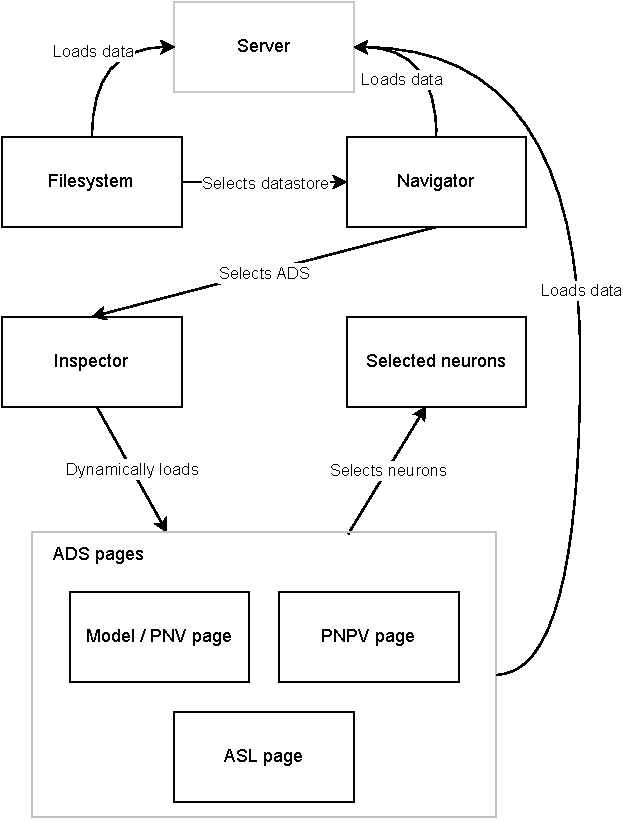
\includegraphics[width=.7\linewidth]{img/frontend_diagram.pdf}
  \caption{Architektura frontendu}
\end{figure}

\begin{figure}
  \centering
  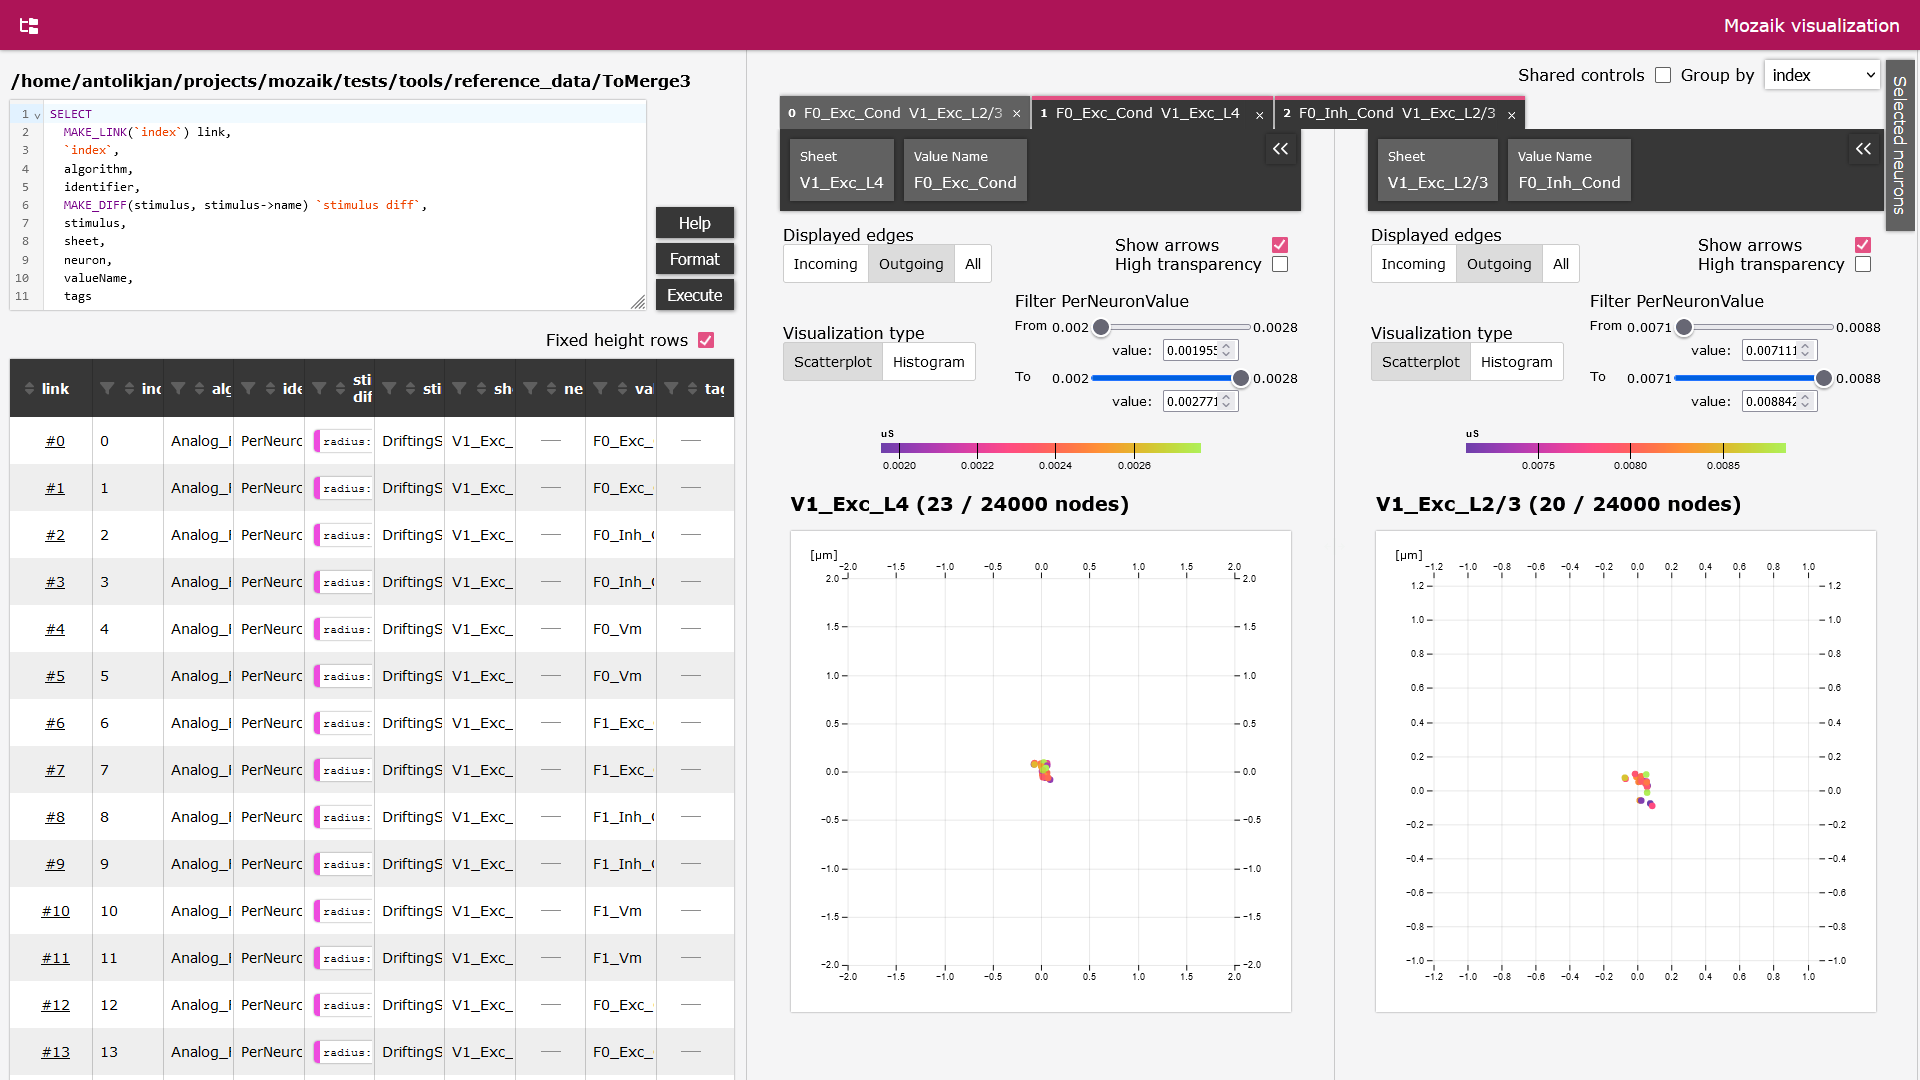
\includegraphics[width=1\linewidth]{img/screenshot_multiview.png}
  \caption{Ukázka upravovatelného layoutu. Na snímku lze vidět nalevo navigátor a napravo inspektor se dvěma aktuálně zobrazenými záložkami. Je možné myší tahat za hranici mezi navigátorem a inspektorem, za hranici mezi záložkami a za hranice mezi jednotlivými sloupci v navigátoru. Je také možné taháním za pravý okraj aplikace zobrazit sidebar s přehledem vybraných neuronů.}
  \label{fig:multiview}
\end{figure}

\subsection{Souborový systém}

Souborový systém zobrazuje složky a datastory. První složky, které uživatel uvidí, jsou nastaveny v konfiguraci a nelze se z nich dostat ven, pouze zanořovat dovnitř. Je možné rekurzivně prohledat celý adresářový strom a získat přehledně zobrazené pouze cesty, na kterých se nějaký datastore nachází. V určitých případech toto může být příliš pomalé, takže je tu ještě klasický způsob postupného zanořování se do složek. Jakmile uživatel zvolí zamýšlený datastore, klient načte základní data --- jednotlivé neuronové vrstvy a spojení a seznam všech ADS.

\subsection{Navigátor}

Navigátor reprezentuje tabulku ADS. Jednotlivé buňky obsahují různé datové typy parametrů, a musí tedy být specializované. Ve stejném sloupci se nicméně předpokládá stejný datový typ, podobně jako v relačních databázích. Jelikož je potřeba mít opravdu silný a robustní způsob vyhledávání, řazení a projekce ADS, je součástí navigátoru SQL editor. Je možné s ADS pracovat, jako by byly uloženy v relační tabulce s podporou pro datový typ JSON. Kromě standardního SQL jsme přidali několik dalších funkcí, které zjednodušují běžnou práci. Více se o nich opět lze dočíst v kapitole \ref{chap:implementation}. SQL jako součást user experience bylo zvolené s ohledem na to, že očekávanými uživateli jsou vývojáři. Pro zjednodušení ale byly přidány i klasické UX prvky. Sloupce lze jedním kliknutím řadit, lze je také filtrovat pomocí specializovaných dialogů. Interně jsou tyto akce nicméně opět převedeny na SQL query. Tyto pomocné filtry a řazení sice stačí po většinu času, na opravdu komplikované dotazy už ale je potřeba SQL měnit ručně.

\subsection{Inspektor}

Inspektor slouží k prohlížení jednotlivých vizualizací. Mezi požadavky na aplikaci je, že musí být možné vybrat několik ADS a mezi nimi rychle přepínat, nebo jich i zobrazit více vedle sebe. Na takovou činnost jsou uživatelé běžně zvyklí například z prohlížeče nebo textových editorů, které používají záložky. Inspektor proto pro co největší intuitivnost používá totéž řešení. Záložky lze řadit, otvírat, zavírat a kombinovat. Pro každou z nich se potom instancuje modul v závislosti na typu ADS. Za načítání doplňujících dat jsou pak zodpovědné právě tyto specializované moduly. 

\subsection{Přehled vybraných neuronů}

Jedná se o komponentu, která zobrazuje seznam právě vybraných neuronů a jejich metadata. Je možné zde výběr i zužovat či rozšiřovat.

\begin{figure}
  \centering
  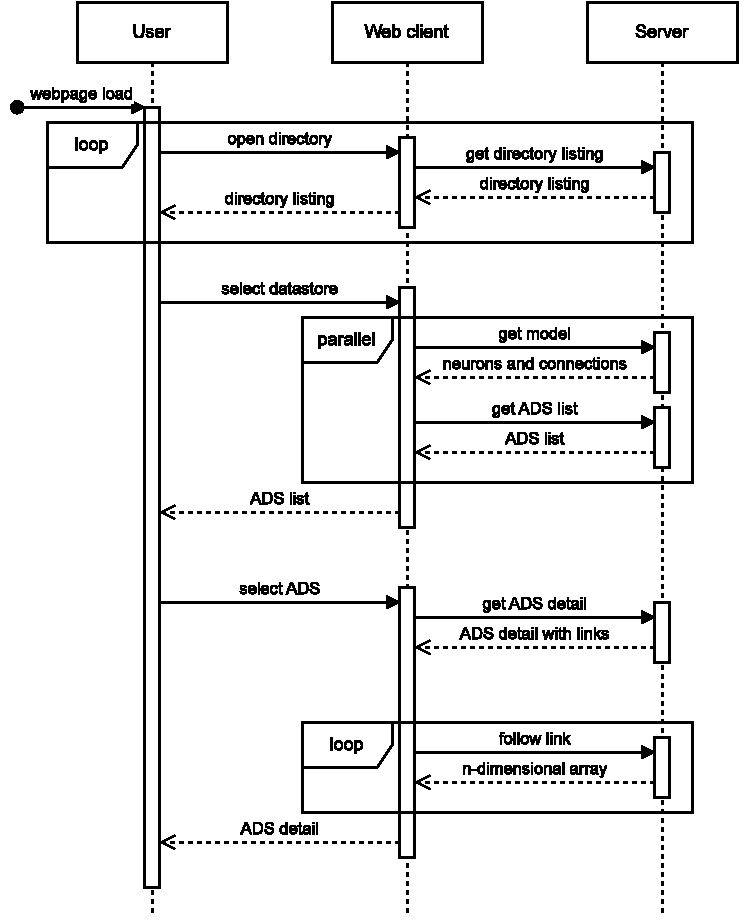
\includegraphics[width=.7\linewidth]{img/ads_sequence.pdf}
  \caption{Příklad komunikace webového klienta a serveru. Po spuštění aplikace je nejprve potřeba vybrat v adresářové struktuře správný datastore. Po jeho zvolení klient načte neuronové vrstvy a jejich spojení a seznam všech ADS. Uživatel si může některou z nich vybrat, tu pak klient načte pomocí jednoho až více dotazů a sestaví kompletní vizualizaci.}
\end{figure}
